% !TEX root = ../KL-Projections.tex


%%%%%%%%%%%%%%%%%%%%%%%%%%%%%%%%%%%%%%%%%%%%%%%%%%%%%
\section{Transport Problems with Ine\-quali\-ty Cons\-traints}

In this section, we consider transport problems with inequality constraints. Again we have to project for the KL divergence on the intersection of convex sets of nonnegative vectors. 


%%%%%%%%%%%%%%%%%%%%%%%%%%%%%%%%%%%%%%%%%%%%%%%%%%%%%%%
\subsection{Partial Transport}
\label{sec-partial-ot}

In the partial transport problem, one is given two marginals $(p,q) \in (\RR_+^N)^2$, not necessarily with the same total mass. 
We wish  to transport only  a given fraction of mass 
\eq{
	m \in [0,\min( p^T\ones, q^T\ones )],  % 	m \in [0,\min( \dotp{p}{\ones}, \dotp{q}{\ones} )],  makes more sense to keep notations consistent.
}
minimizing the transportation cost $\dotp{C}{\pi}$ where $C \in (\RR_+)^{N \times N}$ is the ground cost. 

The corresponding regularized problem reads
% among plans which are consistent with this new constraint introduced as $\Cc_3$ below. 
\eql{\label{partialdiscrete}
	\min_{\pi\in \RR_+^{N\times N}}  
	\enscond{ 
			\dotp{C}{\pi} - \ga E(\pi)
		}{ 
			\pi \ones \leq p, \; 
			\transp{\pi} \ones \leq q, 
			\transp{\ones} \pi \ones = m 
		}
}
where the inequalities should be understood component-wise.

Similarly to~\eqref{eq-regul-ot-kl}, this is equivalent to computing the projection of $\xi=e^{-\frac{C}{\ga}}$ on the intersection $\Cc_1 \cap \Cc_2 \cap \Cc_3$ of $K=3$ convex sets where
\eql{\label{defdesCkpartial}
	\Cc_1 \eqdef \enscond{ \pi }{ \pi \ones \leq p }, \quad
	\Cc_2 \eqdef \enscond{ \pi }{ \transp{\pi} \ones \leq q }, \quad
	\Cc_3 \eqdef \enscond{  \pi }{ \transp{\ones} \pi \ones = m  }.
}
The following proposition shows that the KL projection onto those three sets can be obtained in closed form. 

\begin{prop}
Let   $\pi\in \RR_{+}^{N \times N}$. Denoting $\pi^k \eqdef \KLproj_{\Cc_k}( \pi)$ for $k \in \{1, 2, 3\}$ where $\Cc_k$ is defined by \eqref{defdesCkpartial}, one has
\begin{align*}
	\pi^1 &= \diag\pa{ \min\pa{ \frac{p}{\pi \ones}, \ones} } \pi, \\
	\pi^2 &= \pi \diag\pa{ \min\pa{ \frac{q}{\transp{\pi} \ones}, \ones} }, \\
	\pi^3 &= \pi \frac{m}{\transp{\ones} \pi \ones}, 
\end{align*}
where the minimum is component-wise.
%\eq{
%	\pi_{i,j}^1=
%	\begin{cases}  
%		\pi_{ij} \mbox{ if }  \sum_{j} \pi_{ij}\leq p_i \\   
%		p_i \frac{\pi_{ij}}{\sum_{j'} \pi_{ij'}}    \mbox{ otherwise}     
%	\end{cases} 
%}
%\eq{
%	\pi_{i,j}^2 = 
%	\begin{cases}  
%		\pi_{ij} \mbox{ if }  \sum_{i} \pi_{ij}\leq q_j \\   
%	q_j \frac{\pi_{ij}}{\sum_{i'} \pi_{i'j}}    \mbox{ otherwise}     
%	\end{cases} 
%}
\end{prop}

Since the considered sets $\Cc_1$ and $\Cc_2$ are convex but not affine, one thus needs to use Dykstra iterations~\eqref{eq-iter-dystra} which are ensured to converge to the solution of~\eqref{partialdiscrete}.

If $\pi^\star$ is the optimal solution of~\eqref{partialdiscrete} and 
\eq{
	p_m \eqdef \pi^\star \ones
	\qandq
	q_m \eqdef \pi^{\star,T} \ones
} 
are  its marginals, then we define the active source $\Ss_m$ and the active target $\Tt_m$ regions as follow
\begin{align*}
     \Ss_m &\eqdef \enscond{x_i }{  (p_m)_i/m \geq \eta }, \\
     \Tt_m &\eqdef \enscond{x_i }{  (q_m)_i/m \geq \eta },
\end{align*}
where $\eta>0$ is a threshold we use to detect the region, namely the active region, where the transported mass is concentrated.  

The continuous partial optimal transport problem has been studied in Caf\-far\-el\-li-McCann \cite{MR2630054} and 
Figalli \cite{MR2592287}. They show in particular that if there exists an hyperplane separating the support of the 
two marginals then the  ``active region" is separated from the ``inactive region" by a free boundary which can be parameterized as a semi concave graph over the
separating hyperplane. This can be observed on the test case presented in Figure~\ref{fig:pt1}.
The computation is performed on an uniform 2D-grid of $N=256\times256$ points in $[0,1]^{2}$, $\ga=10^{-3}$ and $m=0.7\min( \dotp{p}{\ones}, \dotp{q}{\ones} )$.
\begin{figure}[htp]
	\centering
	\begin{tabular}{@{}c@{\hspace{1mm}}c@{\hspace{1mm}}c@{}}
		\imgbox{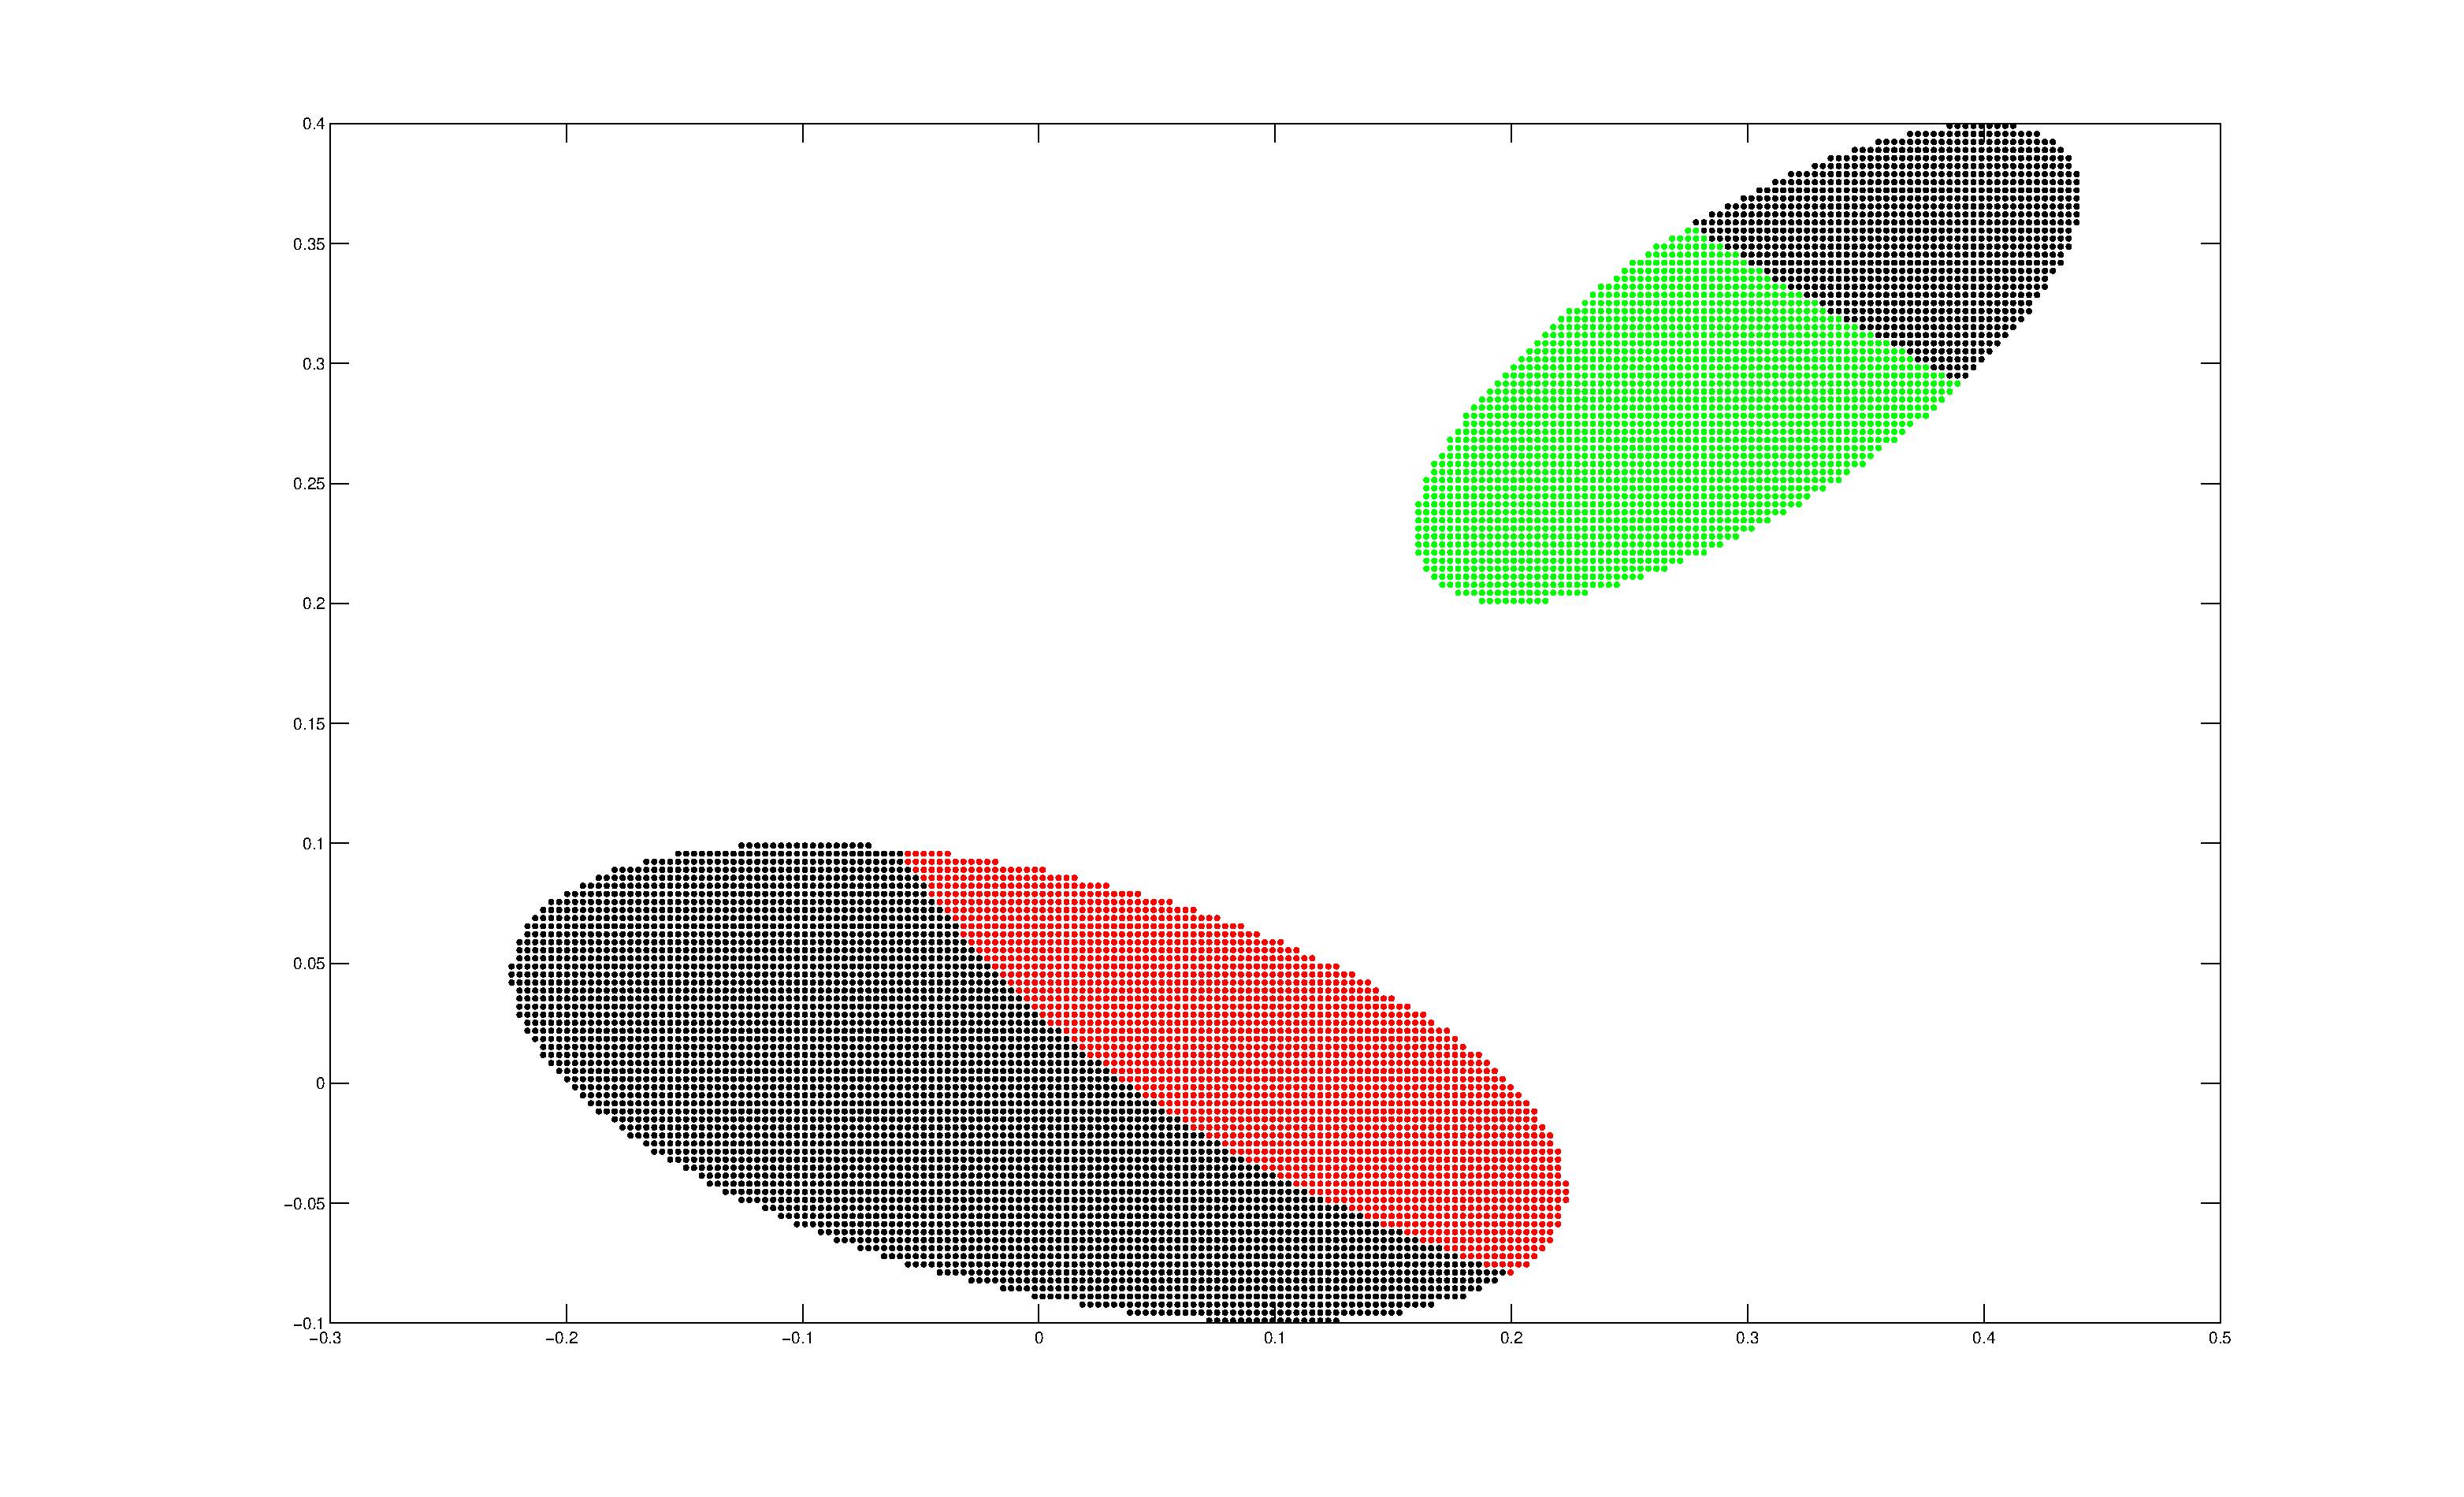
\includegraphics[width=.3\textwidth]{partial/PartialEllipse}} & 
		\imgbox{\includegraphics[width=.3\textwidth]{partial/PartialAnnulusEllipse}} & 
		\imgbox{\includegraphics[width=.3\textwidth]{partial/PartialAnnulusDiamond}} 
	\end{tabular}
  	\caption{ 		�
		The red region is the active source $\Ss_m$, the green region is the active target $\Tt_m$ and the black ones are the inactive regions.
	} 
  	\label{fig:pt1}
\end{figure}

%\begin{figure}[htp]
%	\centering
%	\fbox{{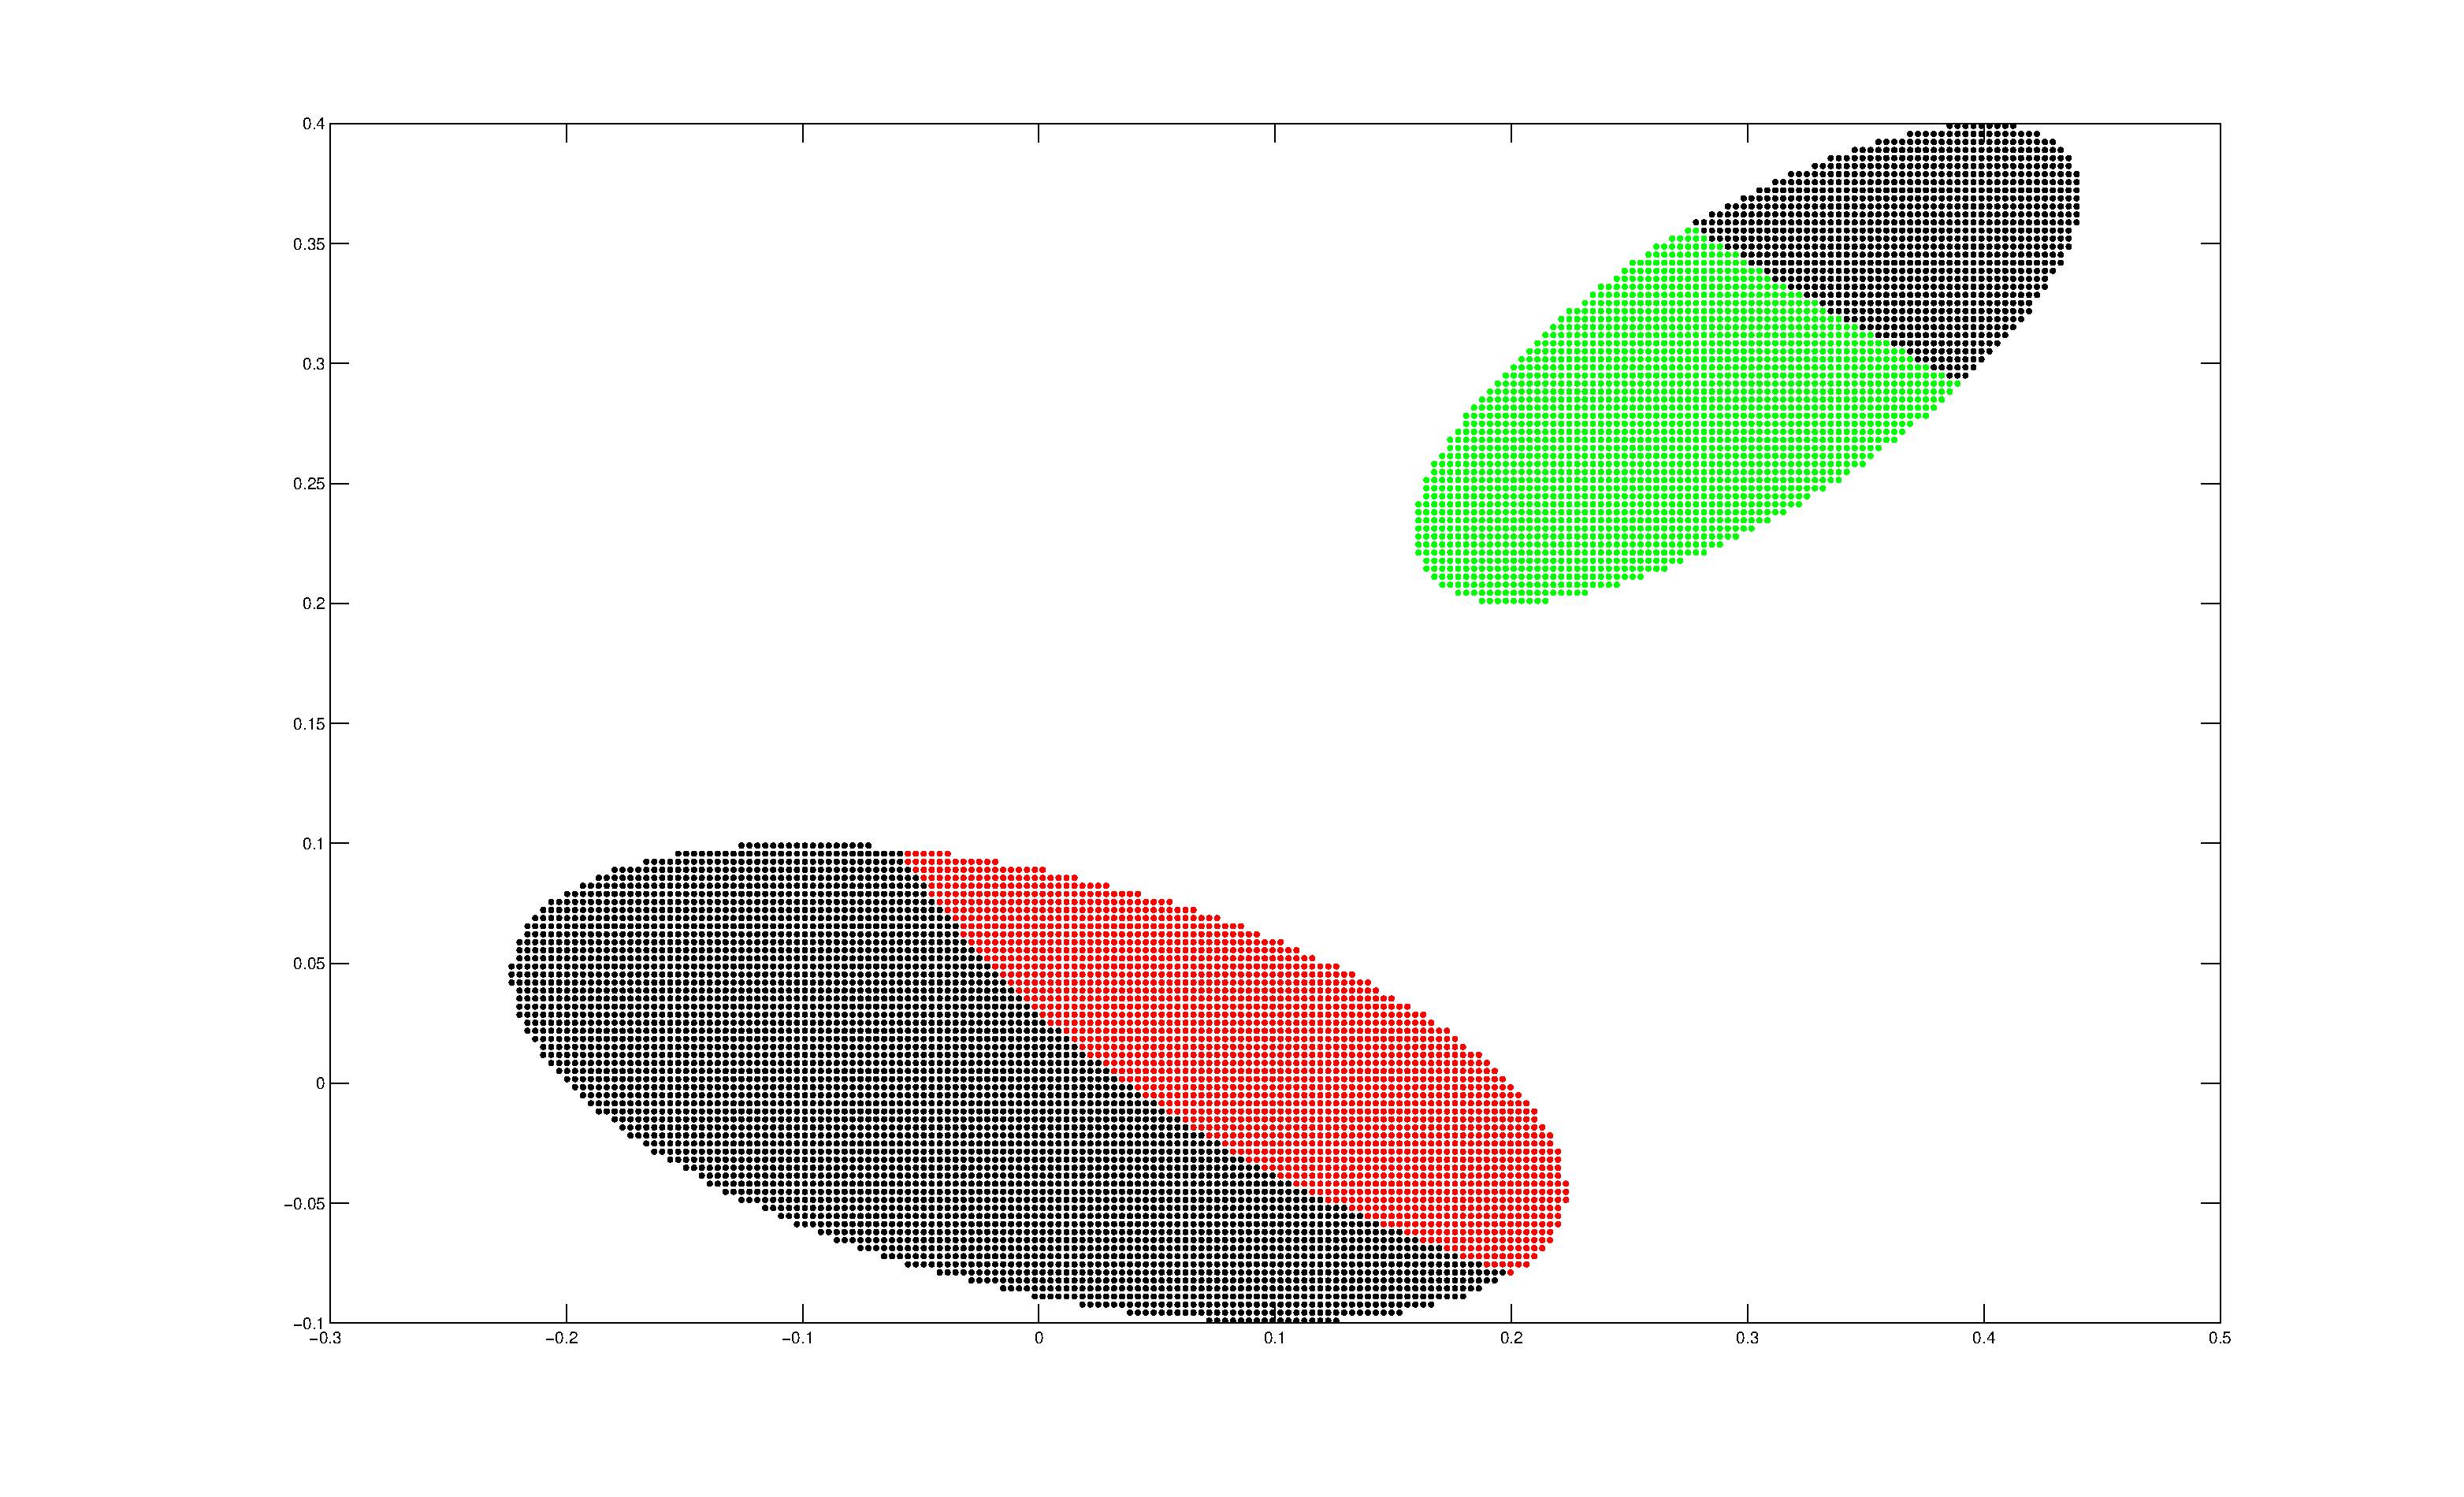
\includegraphics[width=.45\textwidth]{partial/PartialEllipse}}}
 % 	\caption{ The red region is the Active Source, the green region is the Active Target and the black ones are the Inactive regions.
%		\todo{To be consistent with the previous figure, 
%			is possible to use (color) images instead of dots ? 
%			and export them as square images using \texttt{imwrite} ?}
%		\todo{Could you give more details, like value of $N$, $\ga$, and explain what are the colors meanings.
%			In particular I can imaging some sort of thresholding has been used to detect the active mass. }
%			Active mass for a partial optimal transport from an Ellipse to another Ellipse shown on the support of each marginal. 
%	 		The analytical solution is unknown. 	
%	 } 
 % 	\label{fig:pt1}
%\end{figure} 


% \todo{Guillaume: suggestions maybe other more funky examples, Luca, the crown and similar stuff, and why not a multi-marginal unbalanced case as well, reducing the size of the picture, we could put three or four examples, no?}. 


%%%%%%%%%%%%%%%%%%%%%%%%%%%%%%%%%%%%%%%%%%%%%%%%%%%%%%%
\subsection{Capacity Constrained Transport}
\label{sec-capacity-ot}


Korman and McCann proposed and studied in~\cite{km1,km2} a variant of the classical OT problem when there is an upper bound on the coupling weights so as to capture transport capacity constraints. The capacity is described by $\bar{\gamma} \in (\RR_+)^{N \times N}$, where $\bar{\gamma}_{i,j}$ is the maximum possible mass that can be transferred from $i$ to $j$. The corresponding regularized problem reads, for a ground cost $C \in (\RR_+)^{N \times N}$ and marginals $(p,q) \in (\RR_+^N)^2$, 
\eql{\label{constraineddiscrete}
	\min_{\pi\in \RR_+^{N\times N}}  
		\enscond{
			\dotp{C}{\pi} - \ga E(\pi)
		}{
			\pi\ones = p, \; 	
			\transp{\pi}\ones = q, \; 
			\pi \leq \bar{\gamma}
		}
}
where the inequalities should be understood component-wise. This problem is equivalent to a KL projection problem of type~\eqref{proj-inter} with $K=3$ convex sets and
\eql{\label{defdesCkconstrained}
	\Cc_1 \eqdef \enscond{ \pi }{ \pi\ones = p }, \quad
	\Cc_2 \eqdef \enscond{ \pi }{ \transp{\pi}\ones = q },   \quad	
	\Cc_3 \eqdef \enscond{ \pi }{ \pi \leq \bar{\gamma} }.
}
The projection on $\Cc_1$ and $\Cc_2$ is given by Proposition~\ref{prop-projkl-row-cols}. The projection on $\Cc_3$ is simply 
\eq{
	\KLproj_{\Cc_3}(\pi) = \min(\pi, \bar{\gamma})
}
where the minimum is component-wise. Here we have to emphasize the difference between continuous and discrete notations for pointwise capacity constraints; in the continuous problem, one looks for an absolutely continuous with respect to Lebesgue's measure plan $\gamma$ and the capacity constraint reads as $\gamma\le \theta$ where $\gamma$ represents a density and $\theta$ the capacity constraint. In the case of uni-dimensional marginals, if we think of the discrete weight $\gamma_{i,j}$ as the mass of a cell of area $1/N^2$,  $\bar{\gamma}_{i,j}$ represents the integral of $\theta$ on this cell, hence $\bar{\gamma}_{i,j}\simeq \theta_{i,j}/N^2$. Korman and McCann~\cite{km2} established several interesting properties of minimizers in the  continuous setting,  in particular, they proved  (theorem 3.3) that optimal plans must saturate the capacity constraint, that is  optimal plans $\pi$  are of the form $\th\, 1_W$, where $1_W$ is the characteristic function of a subset $W$ of $\RR^d \times \RR^d$. For the quadratic transport cost, uniform marginals  and a constant maximal capacity constraint $\theta$, they also prove  symmetry properties between minimizers  $\pi^\star$, $\tilde\pi^{\star}$ with the same marginals but  different capacity constraints  $\th$ and $\tilde\th$  which are H\"older conjugate, i.e. $\frac{1}{\th} + \frac{1}{\tilde\th} = 1$. More precisely, assuming for simplicity that the marginals are symmetric with respect to 0, they show that 
\begin{equation} 
	\label{sym}
	\pi^\star  = \th\, 1_W   \iff
	\tilde\pi^\star  = \tilde\th\, 1_{R( \Omega \setminus W)}
\end{equation} 
 where $R(x,y) = (x,-y)$ is the symmetry with respect to the second marginal axis and $W$ the optimal support of the saturated constraint 
 $\Cc_3$.
 
 
 
\newcommand{\figCapacity}[1]{\imgbox{\includegraphics[width=.28\textwidth]{capacity/#1}}}

\begin{figure}[htp]
	\centering
	\TabThree{
		\figCapacity{Constrained15} & 
		\figCapacity{Constrained3} & 
		\figCapacity{Constrained2} \\
		$\theta=3/2$ & $\theta=3$ & $\th=2$
	}
  	\caption{ 		�
		Comparison of optimal couplings $\pi^\star$ for different values of $\th$. 	The saturated region $W$ is represented in black.	
	} 
  	\label{fig:cc1}
\end{figure} 


% Figure~\ref{fig:cc3} shows results for the ground cost $C_{i,j} = -x_i \, x_j$ for several values of $\th$ values (that are spacialy constant). 


\begin{figure}[htp]
	\centering
	\TabThree{	
		\figCapacity{Constrained2D151} &
		\figCapacity{Constrained2D152} &
		\figCapacity{Constrained2D153} \\		
		\figCapacity{Constrained2D31} &
		\figCapacity{Constrained2D32} &
		\figCapacity{Constrained2D33}  \\
		$(i_2,j_2)=(\frac{\sqrt{N}}{4},\frac{\sqrt{N}}{4})$ &
		$(i_2,j_2)=(\frac{\sqrt{N}}{2},\frac{\sqrt{N}}{2})$ &
		$(i_2,j_2)=(\frac{3\sqrt{N}}{4},\frac{3\sqrt{N}}{4})$ \\
	}
  	\caption{ 
		2-D slices of the optimal coupling $\pi^\star$ 
		of the form $(\pi^\star_{(i_1,i_2)(j_1,j_2)})_{i_1,j_1}$, each time for 
		some fixed value of $(i_2,j_2) \in \{1,\ldots,\sqrt{N}\}^2$, 
		for $\th=3/2$ (top row) and $\th=3$ (bottom row).
	} 
  	\label{fig:cc3}
\end{figure} 

 
Korman and McCann~\cite{km2} illustrated their theory with two 1-D numerical test cases (Figures 1 and 2 of~\cite{km2}) computed by linear programming and a discretization of the problem on a cartesian grid. We tested our method on the same examples. 
%
The ground cost is the standard quadratic distance $C_{i,j} = \norm{x_i-x_j}^2$, the marginals are discretizations of the uniform distribution on $[-1/2,1/2]$ using $N=100$ points $(x_i)_{i}$.
%
The simulation uses $\ga=10^{-3}$.
% 
We reproduce the expected symmetries~\eqref{sym} in Figure~\ref{fig:cc1} in the 1-D test case for $\th=\frac{3}{2}$  and $\tilde\th=3$ and also for the self dual H\"older conjugate $\th=\tilde\th=2$.   

% \todo{Why using notation $(k^*,k^{**})$ and not simply $(k,k^*)$ ? The following is not clear to me.}

We also computed the solutions of similar test cases but this time in 2-D, which would be computationally too expensive to solve with linear programming methods.
%
The marginals $(p,q)$ are discretization of the uniform distribution on the square $[-1/2,1/2]^2$, discretized on a grid of $N=50 \times 50$ points $(x_i)_i$.
%
The simulation uses $\ga=10^{-3}$.
%
Figure~\ref{fig:cc3} shows some slices of the 4-D array representing the optimal transport plan $\pi^\star$, $\tilde\pi^\star$, illustrating the symmetries~\eqref{sym} in this setting.


% In order to visualize the transport plans, we fix $k=k^*$ (and $\ell=\ell^*$) and \todo{Gabriel: I did not understood what is actually plot, since $\pi^\star_{i,j,k^*,\ell^*}$ is a real number. Also one should rather use notation of the form $\pi_{(i_1,i_2),(j_1,j_2)} = \pi_{i,j}$ where $i,j$ are couples of $(x,y)$ variables. }�we plot $\pi^\star_{i,j,k^*,\ell^*}$ and $\tilde\pi^\star_{i,j,k^{**},\ell^{**}}$ where $k^{**}=N-k^*+1$ ($\ell^{**}=N-\ell^*+1$) to check the symmetry~\eqref{sym}. Figure~\ref{fig:cc3} shows slices  of the 4-D  transport plans $\pi^\star$, $\tilde\pi^\star$ , the symmetry property~\eqref{sym} is satisfied. 




%%%%%%%%%%%%%%%%%%%%%%%%%%%%%%%%%%%%%%%%%%%%%%%%%%%%%%%%%%%%%%%%%%%
\subsection{Multi-Marginal Partial Transport} 


In~\cite{passkitagawa} Pass and Kitagawa studied the multi-marginal partial transport problem and, as a natural extension, the partial barycenter problem. Let us consider $K$ marginals $(p_k)_{k=1}^{K}$ and a transport plan $\pi \in \RR_{+}^{N^K}$.
We now combine the (regularized) partial optimal transport and the ``standard" multi-marginal problem, as described
in Sections~\ref{sec-partial-ot} and~\ref{subsec-multi-marginal-regularization} respectively. We obtain the following problem
\eql{\label{eq-partial-multimarginal-proj}
	\min_\pi \enscond{
		\KLdiv{\pi}{\xi} 
	}{
		\pi \in \Cc_1 \cap \Cc_2 \cap \ldots \cap \Cc_{K+1}
	}
	\qwhereq
	\xi \eqdef e^{-\frac{C}{\ga}}
}
where

\begin{align*}
	\Cc_k &\eqdef \enscond{ \pi \in \RR_+^{N^K} }{�S_k(\pi) \leq \km{p} }\quad k=1,\ldots,K, \\
	\Cc_{K+1} &\eqdef \enscond{ \pi \in \RR_+^{N^K} }{\textstyle \sum_{j}\pi_{j}=m},
\end{align*}
with $m \in [0,\min_k(\dotp{p_k}{\ones})]$

The KL projections on these convex sets are detailed in the following proposition.

\begin{prop}%\todo{The equations for these projections were wrong, double check what I wrote instead.}
	For any $k = 1,\ldots,K+1$, denoting $\pi^k = \KLproj_{\Cc_k}(\bar\pi)$, one has 
	\eq{
		\foralls k=1,\ldots,K, \; 
		\foralls j=(j_1,\ldots,j_K), \quad		
		\pi_{j}^k = \min\pa{ \frac{(\km{p})_{j_k}}{ S_k(\bar\pi)_{j_k} },1 } \bar\pi_{j}�
	}
	\eq{		
		\pi^{K+1} =\frac{m}{ \sum_{j}\bar\pi_{j} } \bar\pi.�
	}
\end{prop}


Once again the sets $\Cc_k$ are not affine, so  one  needs to use Dykstra iterations~\eqref{eq-iter-dystra}.

Figure~\ref{fig:pmm1} shows the results obtained when solving~\eqref{eq-partial-multimarginal-proj} with the same three marginals $(p_1,p_2,p_3)$ used in Figure~\ref{fig-barycenter-entropic}, using the cost 
\eql{\label{partial-quadratic-standard}
	C_{j_1,j_2,\ldots,j_K}  = \sum_{1 \leq s,t \leq K}\dfrac{1}{2} \norm{ x_{j_s}-x_{j_t} }^2, 
}
The computation is performed on an uniform 2D-grid of $N=60\times60$ points in $[0,1]^2$, $\ga=0.005$ and $m=0.7\min_k(\dotp{p_k}{\ones})$.


% This figure compares two different ground costs $C$, the ``standard" quadratic cost for the multi-marginal problem
%\eql{\label{partial-quadratic-standard}
%	C_{j_1,j_2,\ldots,j_K}  = \sum_{1 \leq s,t \leq K}\dfrac{1}{2} \norm{ x_{j_s}-x_{j_t} }^2, 
%}
%and the cost associated to the barycenter problem 
%\eql{\label{partial-barycenter}
%	C_{j_1,j_2,\ldots,j_K}  = \sum_{1 \leq s \leq K}\dfrac{\lambda_{s}}{2} \norm{ x_{j_s}-A_j(x) }^2.  % ,\, j_i \ne j_i'
%}
%We refer to Section~\ref{sec-multi-marginal} for details about how the display of the barycenter measure is performed.
%


\newcommand{\figMultiPartial}[1]{\imgbox{\includegraphics[width=.4\textwidth]{multimarginal/PartialMultimarginal/#1}}}

\begin{figure}[htp]
	\centering
%	\TabTwo{	
		\figMultiPartial{PartialAnnulusDiamondSquare} % &
%		\figMultiPartial{PartialBar} \\
 %           Cost~\eqref{partial-quadratic-standard} & Cost~\eqref{partial-barycenter}
%
%	}
  	\caption{
		Multi-marginal partial transport.
		The active regions are displayed in red. 
	} 
  	\label{fig:pmm1}
\end{figure}


